% ============================================================== PART I
\section{Two compressions}\label{sec:two}

\subsection{The black hole interior}\label{sec:bh}
The literature on the quantum mechanics of black holes is enormous; the part we need concerns Hawking's information
paradox and its recent resolution through holography~\cite{Penington,AEMM,AEHPV}. In particular, we exploit the
insight of Akers, Engelhardt, Harlow, Penington and Vardhan~\cite{AEHPV} that the effective description of the
black hole interior---the ``bulk'' local physics, such as the creation and annihilation operators of quantum fields
inside the horizon---is related to the fundamental description by a random linear compression. The fundamental
description consists of the black hole's own remaining degrees of freedom, counted by its entropy, together with the
radiation it has emitted; the compression acts on the interior modes alone and carries the radiation across
untouched (\cref{fig:penrose}). This single picture accounts for several pieces of black hole folklore: the Page
curve of the radiation entropy, the state-dependence of interior operators, the absence of low-complexity null
states, and the exponential cost of decoding the radiation.

\begin{figure}[t]
\centering\PenroseSlice
\caption{Late-time Cauchy slice $\Sigma_t$ of an evaporating black hole formed by a collapsing shell (zoomed on the
relevant region; null lines at $45^\circ$). Outside the horizon the slice carries the outgoing Hawking modes $r$,
which are the same system $R$ in both descriptions. Inside, it carries the infalling partner modes $\ell$ near the
horizon and, at its inner end, the collapsed matter $f$, frozen in the state it fell in with. In the fundamental
description the whole interior segment is encoded in the black hole's microstates $B$ at the horizon crossing, with
$\dim\Hil_B=e^{A/4G}$: the map $V$ squeezes a segment onto a point whose size is its area. Lower-case labels are
what a semiclassical observer assigns to a region; upper-case labels are the fundamental Hilbert spaces. They differ
only at the horizon, and the difference is $V$.}
\label{fig:penrose}
\end{figure}

Formally, we can forget about gravity and time evolution and focus on the linear algebra of inner-product spaces.
The effective description of the interior is a Hilbert space $\Hil_\ell$ of dimension $\abs{\ell}=e^{S_\ell}$; at
late times $S_\ell$ exceeds the black hole's Bekenstein--Hawking entropy $S_{\rm BH}$, because the interior keeps
growing while the black hole shrinks. The fundamental description of the black hole is $\Hil_B$ with
$\abs{B}=e^{S_{\rm BH}}$. The two are related by
\begin{equation}\label{eq:V}
V\colon\Hil_\ell\to\Hil_B,\qquad V=\sqrt{\abs{P}}\;\bra{0}_P\,U\,\ket{\psi_0}_f ,\qquad \abs{\ell}\abs{f}=\abs{B}\abs{P},
\end{equation}
extended by the identity on the radiation. Here $U$ is a Haar-random unitary on $\Hil_\ell\otimes\Hil_f$ standing
in for the unknown, scrambling dynamics; $f$ is the collapsed matter, prepared in a fixed state $\ket{\psi_0}$ by the
history of the collapse; and $P$ is a bookkeeping remainder. The interior $\ell\otimes f$ has more states than the
black hole $B$ can hold, so the unitary must output them somewhere: $P$ is that somewhere, discarded by projection
onto $\ket 0_P$---the states the black hole would have needed had it not shrunk.

The factor $\sqrt{\abs P}$ makes typical states come out with unit norm. Indeed
$\bra0_PU\ket{\psi_0}_f$ is a block of $U$, and $U^\dagger(I_B\otimes\ket0\bra0_P)U$ is a Haar-random projector of
rank $\abs B$ on a space of dimension $\abs\ell\abs f=\abs B\abs P$, so by \cref{lem:projectors},
$\E\,V^\dagger V=\abs P\cdot\frac{\abs B}{\abs\ell\abs f}\,I_\ell=I_\ell$.

For the linear algebra the ancillae are inessential and we use the \emph{reduced model} $\abs f=1$:
\begin{equation}\label{eq:reduced}
V=\sqrt{M/N}\;P_NU,\qquad M=\abs\ell,\ N=\abs B,
\end{equation}
$\sqrt{M/N}$ times $N$ rows of a Haar unitary. Then $V^\dagger V=\frac MN Q$ with $Q$ a Haar-random rank-$N$
projector. Since $M>N$, $\dim\ker V\ge M-N$: almost all of the effective space consists of \emph{null states}
that the fundamental description cannot distinguish from zero. The content of~\cite{AEHPV} is that $V$ is
nonetheless an isometry to any observer of bounded complexity; \cref{sec:theorem} proves the version we need.

\subsection{Superposition}\label{sec:superposition}
The working hypothesis of mechanistic interpretability is that a trained network computes with \emph{features}:
directions in activation space that correspond to human-legible properties of the input. The obstacle is that
features are not neurons. A neuron typically responds to several unrelated features and a feature is spread across
many neurons---\emph{polysemanticity}. Elhage et al.~\cite{TMS} showed that polysemanticity is what compression
looks like from the inside. A network that must represent $m$ features in $n<m$ neurons can, if the features are
sparse, assign each a direction in $\R^n$ and accept that the directions overlap, because overlaps only matter
when overlapping features are simultaneously active. This is \emph{superposition}: the network simulates a larger,
monosemantic network (\cref{fig:tms}).

\begin{figure}[t]
\centering\TMSPicture
\caption{Superposition. Left: $m$ features feed $n<m$ neurons; a sparse input (shaded) activates few features but
every neuron reads several. Right: the classic toy-model solution with $m=5$ features in $n=2$ dimensions, a
regular pentagon~\cite{TMS}.}
\label{fig:tms}
\end{figure}

The effective description is feature space $\R^m$; a feature activation $x$ is nonzero on few coordinates, and we
write $\Sigma_k$ for the unit vectors with at most $k$ nonzero entries. The fundamental description is the
activation space $\R^n$. The two are related by $W\colon\R^m\to\R^n$, $h=Wx$, whose columns $w_1,\dots,w_m$ are the
feature directions. In the toy models of~\cite{TMS} the readout is $\hat x=\ReLU(W^\top h+b)$. The transpose alone
cannot undo superposition (any linear map $\R^n\to\R^m$ has rank $\le n$); $W^\top Wx=x+e$ is correct on the active
coordinates up to the \emph{interference} $e_i=\sum_{j\ne i}\ip{w_i}{w_j}x_j$, and the ReLU with negative bias
projects back onto the sparse set by thresholding the interference away (\cref{prop:onestep}). Since $m>n$, $W$
cannot be an isometry; its kernel contains the dense activation patterns that a sparse network never produces.

\subsection{The static dictionary}
\Cref{tab:static} lines up the two settings. The quantitative content of ``preserves inner products on a
distinguished set'' is the subject of \cref{sec:theorem}. The one structural asymmetry is that $V$ is assembled
from a unitary with ancillae, because in gravity the scrambling is unitary and the compression has to be
manufactured from it, whereas $W$ is trained directly; nothing in the dictionary depends on the ancillae.

\begin{table}[h]
\centering\small
\begin{tabular}{@{}lll@{}}
\toprule
 & black hole (AEHPV) & network (superposition) \\
\midrule
effective space & interior $\Hil_\ell$, $\dim=e^{S_\ell}$ & features $\R^m$ \\
fundamental space & microstates $\Hil_B$, $\dim=e^{S_{\rm BH}}$ & neurons $\R^n$ \\
code & $V$, from a Haar unitary & $W$, trained (Haar as baseline) \\
null space & $\dim\ge M-N$, all high complexity & $\ker W$, no $k$-sparse vectors \\
distinguished set & complexity $\le C$ & $k$-sparse \\
its size & $\log\abs{\Sigma_C}\lesssim C\log S_\ell$ & $\log\binom mk\le k\log(em/k)$ \\
overlap fluctuations & $\approx e^{-S_{\rm BH}/2}$ & $\approx n^{-1/2}$ \\
field & $\C$ ($\beta=2$) & $\R$ ($\beta=1$) \\
\bottomrule
\end{tabular}
\caption{The static dictionary. The exponential in the left column becomes polynomial on the right:
$e^{S_{\rm BH}}\leftrightarrow n$, hence $S_{\rm BH}\leftrightarrow\log n$.}
\label{tab:static}
\end{table}

% --------------------------------------------------------------------------
\section{The unifying theorem}\label{sec:theorem}

Throughout, a code maps an $M$-dimensional effective space to an $N$-dimensional fundamental space over
$\F\in\{\R,\C\}$; write $\beta=\dim_\R\F$. The \emph{Haar code} is $V=\sqrt{M/N}\,P_NU$ with $U$ Haar on $U(M)$
(complex) or $O(M)$ (real); in the real case we write $W$, $m$, $n$. For a set $\Sigma$ of unit vectors the
distortion is $\epsilon_\Sigma(V)=\sup_{x,y\in\Sigma}\abs{\ip{Vx}{Vy}-\ip xy}$.

\subsection{Second moments}
\begin{lemma}[Projector moments]\label{lem:projectors}\proved
Let $Q$ be a Haar-random rank-$N$ orthogonal projector on $\F^M$. Then $\E Q=\frac NM I$, and
\begin{align*}
\F=\C:&\quad \E[Q\otimes Q]=aI+bF, & a&=\tfrac{N(NM-1)}{M(M^2-1)},\ \ b=\tfrac{N(M-N)}{M(M^2-1)};\\
\F=\R:&\quad \E[Q\otimes Q]=\alpha I+\gamma(F+\Omega), & \gamma&=\tfrac{N(M-N)}{M(M-1)(M+2)},\ \ \alpha=\tfrac NM-\gamma(M+1),
\end{align*}
where $F$ is the swap and $\Omega=\ket\omega\bra\omega$ with $\ket\omega=\sum_ie_i\otimes e_i$.
\end{lemma}
\begin{proof}
$\E Q$ commutes with every unitary (orthogonal) $g$, since $g^\dagger Qg$ has the same law as $Q$; so $\E Q=cI$ and
$\tr$ gives $c=N/M$. Likewise $\E[Q\otimes Q]$ commutes with all $g\otimes g$. Over $\C$ the commutant of
$\{g\otimes g\}$ is spanned by $I,F$ (Schur--Weyl); over $\R$ by $I,F,\Omega$ (Brauer). Fix the coefficients by
traces. Over $\C$: $\tr\E[Q\otimes Q]=(\tr Q)^2=N^2=aM^2+bM$ and $\tr(F\,\E[Q\otimes Q])=\tr Q^2=N=aM+bM^2$, which
solve to the stated $a,b$. Over $\R$ there is a third equation, $\tr(\Omega\,\E[Q\otimes Q])=\tr(QQ^\top)=N$; using
$\tr F=\tr\Omega=M$, $\tr(F\Omega)=M$, $\tr F^2=\tr\Omega^2=M^2$, the second and third equations are symmetric in the
coefficients of $F$ and $\Omega$, so these are equal ($=\gamma$), and $N^2=\alpha M^2+2\gamma M$,
$N=\alpha M+\gamma(M^2+M)$ give $\gamma M(M-1)(M+2)=N(M-N)$.
\end{proof}

\begin{proposition}[Exact overlap variances]\label{prop:variances}\proved\ \numchk
For fixed unit vectors with overlap $c$, $\E\ip{Vx}{Vy}=c$ and
\[
\Var_{\C}=\frac{(M-N)(M-\abs c^2)}{N(M^2-1)},\qquad
\Var_{\R}=\frac{(m-n)\,\big(m+(m-2)c^2\big)}{n\,(m-1)(m+2)},\qquad
\Var_{\rm Gauss}=\frac{1+c^2}{n},
\]
the last for i.i.d.\ $\mathcal N(0,1/n)$ entries. For $N\ll M$ the complex variance is $\approx1/N$ independently of
$c$; the real one is $\approx(1+c^2)/n$, and the extra $c^2$ is exactly the $\Omega$ term of \cref{lem:projectors},
the Brauer invariant that is present for $O(n)$ and absent for $U(n)$. Haar frames beat Gaussian ones by a factor
$\approx(1-n/m)$.
\end{proposition}
\begin{proof}
$\E\abs{\bra x Q\ket y}^2=(\bra x\otimes\bra y)\E[Q\otimes Q](\ket y\otimes\ket x)=a\abs c^2+b$ over $\C$; over $\R$,
$\E(x^\top Qy)^2=(\alpha+\gamma)c^2+\gamma$. Multiply by $(M/N)^2$, subtract $\abs c^2$, simplify. For Gaussian
entries apply Isserlis to the $n$ independent terms $\ip{g_i}x\ip{g_i}y$.
\end{proof}

\begin{proposition}[Frame identity]\label{prop:frame-identity}\proved
Let $w_1,\dots,w_m$ be unit vectors in $\R^n$ forming a tight frame ($WW^\top=\frac mn I$). Then
\[
\frac{1}{m(m-1)}\sum_{i\ne j}\ip{w_i}{w_j}^2=\frac{m-n}{n(m-1)} .
\]
Hence \emph{every} unit-norm tight frame agrees with the Haar prediction $\frac{m(m-n)}{n(m-1)(m+2)}$ for the
mean-square interference, up to a factor $m/(m+2)$.
\end{proposition}
\begin{proof}
$\sum_{i,j}\ip{w_i}{w_j}^2=\norm{W^\top W}_F^2=\norm{WW^\top}_F^2=(m/n)^2n$; subtract the $m$ diagonal terms.
\end{proof}
This matters for experiments: agreement with Haar at second order is evidence of tightness, not of randomness.

\subsection{Concentration and the theorem}
\begin{lemma}[Law of a compressed norm]\label{lem:beta}\proved
For fixed unit $z$, $\norm{Vz}^2\overset{d}{=}\frac MN\cdot\frac{A}{A+B}$ with $A\sim\chi^2_{\beta N}$,
$B\sim\chi^2_{\beta(M-N)}$ independent.
\end{lemma}
\begin{proof}
$\norm{Vz}^2=\frac MN\norm{P_NUz}^2$ and $Uz$ is uniform on the unit sphere of $\F^M\cong\R^{\beta M}$, i.e.\ $g/\norm
g$ with $g$ standard Gaussian. $\norm{P_Ng}^2\sim\chi^2_{\beta N}$ and $\norm{(1-P_N)g}^2\sim\chi^2_{\beta(M-N)}$
independently.
\end{proof}

\begin{lemma}[$\chi^2$ concentration]\label{lem:chisq}\proved
For $Z\sim\chi^2_k/k$ and $0<s\le1$: $\Pr[\abs{Z-1}\ge s]\le2e^{-ks^2/12}$.
\end{lemma}
\begin{proof}
Chernoff with $\E e^{\lambda\xi^2}=(1-2\lambda)^{-1/2}$. Upper tail: $\lambda=\frac{s}{2(1+s)}$ gives exponent
$-\frac k2[s-\log(1+s)]\le-\frac{k}{2}(\frac{s^2}{2}-\frac{s^3}{3})\le-\frac{ks^2}{12}$. Lower tail:
$\lambda=\frac{s}{2(1-s)}$ for the variable $-\xi^2$ gives exponent $-\frac k2[-s-\log(1-s)]\le-\frac{ks^2}{4}$.
\end{proof}

\begin{theorem}[Random codes are isometries on thin sets]\label{thm:main}\proved
Let $V$ be the Haar code over $\F$ and $T$ a finite set of unit vectors. For $0<\delta\le1$,
\[
\Pr\Big[\sup_{z\in T}\big|\norm{Vz}^2-1\big|>\delta\Big]\le4\abs T\,e^{-\beta N\delta^2/108}.
\]
Consequently, for any finite set $\Sigma$ of unit vectors, $\epsilon_\Sigma(V)\le2\delta$ with probability at least
$1-16\abs\Sigma^2e^{-\beta N\delta^2/108}$; that is, the code is an approximate isometry on $\Sigma$ as soon as
\begin{equation}\label{eq:condition}
\boxed{\;\log\abs\Sigma\;\ll\;\beta\,N\,\delta^2\;}
\end{equation}
\end{theorem}
\begin{proof}
By \cref{lem:beta}, $\norm{Vz}^2=\frac{A/\beta N}{(A+B)/\beta M}$. If numerator and denominator are both within
$1\pm\delta/3$ the ratio is within $1\pm\delta$ (since $\frac{1+t}{1-t}\le1+3t$ for $t\le\frac13$), and by
\cref{lem:chisq} each fails with probability at most $2e^{-\beta N\delta^2/108}$. Union-bound over $T$. For the
second statement apply this to $T=\{(x+\omega y)/\norm{x+\omega y}\}$ with $\omega\in\{\pm1\}$ (real) or
$\{\pm1,\pm i\}$ (complex), $\abs T\le4\abs\Sigma^2$, and use polarization:
$\abs{\ip{Vx}{Vy}-\ip xy}\le\frac14\sum_\omega\delta\norm{x+\omega y}^2\le2\delta$.
\end{proof}

The theorem never asks which field or which set it is given; it sees only $\beta$ and $\log\abs\Sigma$. Its two
specializations are the two halves of the correspondence.

\begin{corollary}[AEHPV: low complexity]\label{cor:aehpv}\proved
Over $\C$ with $N=e^{S_{\rm BH}}$, let $\Sigma_C$ be the states preparable from a fixed reference state by circuits of
at most $C$ gates from a finite gate set $G$ acting on the $S_\ell$ interior qubits. Then
$\abs{\Sigma_C}\le(\abs G S_\ell^2)^C$, and with high probability
\[
\sup_{\psi,\phi\in\Sigma_C}\big|\bra\psi V^\dagger V\ket\phi-\braket\psi\phi\big|\lesssim\sqrt{C\log S_\ell}\;e^{-S_{\rm BH}/2},
\]
negligible for all $C$ sub-exponential in $S_{\rm BH}$. In particular no state of sub-exponential complexity is null.
\end{corollary}

\begin{corollary}[Restricted isometry]\label{cor:rip}\proved
Over $\R$, $W$ satisfies $(1-\delta)\le\norm{Wx}^2\le(1+\delta)$ for all $k$-sparse unit $x$ with high probability
once $n\gtrsim\delta^{-2}k\log(em/k)$.
\end{corollary}
\begin{proof}
For each support $S$ take an $\eta$-net of the unit sphere of $\R^S$ with at most $(3/\eta)^k$ points; the union
over $\binom mk$ supports has $\log\abs T\le k\log(em/k)+k\log(3/\eta)$. Apply \cref{thm:main} to the net, then
extend from the net to the sphere: if $1-\delta'\le\norm{Wz}\le1+\delta'$ on the net and $A=\sup\norm{Wz}$, then
$A\le1+\delta'+\eta A$, so $A\le(1+\delta')/(1-\eta)$, and similarly from below; take $\eta=\delta'/4$.
\end{proof}

\begin{remark}[No simple null vectors]
If $\delta_{2k}<1$ then no nonzero $2k$-sparse vector is in $\ker W$, so $\spark(W)>2k$ and each $k$-sparse vector
is determined by its image. The dictionary entry is: $\spark(W)$ is the complexity of the cheapest null state.
\end{remark}

\begin{remark}[Gaussian width]\label{rem:width}\cited
The finite-set condition $\log\abs\Sigma\ll\beta N\delta^2$ is the special case of Gordon's
theorem~\cite{Gordon,Vershynin}: a Gaussian $n\times m$ map is an approximate isometry on any $T\subset S^{m-1}$
with distortion $\lesssim w(T)/\sqrt n$, where $w(T)=\E\sup_{z\in T}\ip gz$. For finite sets $w(T)\le\sqrt{2\log\abs
T}$ (Jensen on $\E\max e^{\lambda\ip gz}$), and for the $k$-sparse sphere
$w(\Sigma_k)\le\sqrt k+\sqrt{2\log\binom mk}$ (the same argument applied to the 1-subgaussian variables
$\norm{g_S}-\E\norm{g_S}$, with $\E\norm{g_S}\le\sqrt k$). Width is the right size for $\Sigma$; low complexity and
sparsity are two ways of having small width. We do not need the complex version of Gordon's theorem, because both
corollaries above go through the finite-set form.
\end{remark}

\begin{remark}[Where the exponential goes]
Gravity compares $\mathrm{poly}(C)$ with $e^{S_{\rm BH}}$; a network compares $k\log(m/k)$ with $n$. The dictionary
is $e^{S_{\rm BH}}\leftrightarrow n$, so corrections that are $e^{-S/2}$ in gravity are $n^{-1/2}$ in a network,
and an effective description that is quasi-exact for a black hole is merely approximate for a transformer. This is
the largest quantitative deflation in passing from one column of \cref{tab:static} to the other.
\end{remark}

% --------------------------------------------------------------------------
\section{The reconstruction dictionary}\label{sec:dictionary}

\subsection{Decoders}
On both sides the naive decoder is the adjoint of the encoder: the Petz (transpose) map~\cite{Petz} in gravity,
$W^\top$ followed by a nonlinearity in a network.
\begin{lemma}\proved
If $\epsilon_\Sigma(V)\le\epsilon$ then $\abs{\ip y{V^\dagger Vx}-\ip yx}\le\epsilon$ for all $x,y\in\Sigma$.
\end{lemma}
That is all one can say: $V^\dagger Vx$ agrees with $x$ against every test vector in $\Sigma$ and may be badly wrong
elsewhere. In a network this ``elsewhere'' is the interference, and the nonlinearity's job is to project back to
$\Sigma$.
\begin{proposition}[One-step thresholding]\label{prop:onestep}\proved
If the columns of $W$ are unit vectors with coherence $\mu=\max_{i\ne j}\abs{\ip{w_i}{w_j}}$ and $x\in\{0,1\}^m$ has
at most $k$ ones, then $\abs{(W^\top Wx)_i-x_i}\le\mu k$; so $\ReLU(W^\top Wx-\frac12)$ followed by rounding
recovers $x$ when $\mu k<\frac12$.
\end{proposition}
For random unit columns $\mu\approx\sqrt{2\log m/n}$, so one step tolerates $k\lesssim\sqrt{n/\log m}$, whereas the
isometry holds up to $k\sim n/\log(m/k)$; iterative and convex decoders close the gap (\cref{sec:page}).

\subsection{State dependence}\label{sec:state-dependence}
\begin{proposition}[Why reconstruction must be state-dependent]\label{prop:statedep}\proved
In the reduced model, for any operator $A$ on the effective space,
\[
\E\big[V^\dagger V\,A\,V^\dagger V\big]=\frac{M(NM-1)}{N(M^2-1)}\,A+\frac{M(M-N)}{N(M^2-1)}\,\tr(A)\,I\;\approx\;A+\frac{\tr A}{N}\,I .
\]
So the state-independent reconstruction $VAV^\dagger$ has, in every state $V\ket\phi$, an expectation biased by
$\approx e^{-S_{\rm BH}}\tr A$. For $A=I$ the reconstruction $VV^\dagger$ has expectation exactly
$\frac MN\bra\phi V^\dagger V\ket\phi\approx e^{S_\ell-S_{\rm BH}}$: the fundamental description of the identity is
not even approximately the identity. A state-dependent reconstruction $A_\phi$ defined by $A_\phi V\ket\phi=VA\ket\phi$
inherits the accuracy of \cref{cor:aehpv} whenever $\ket\phi$, $A\ket\phi$ and $B\ket\phi$ are low-complexity.
\end{proposition}
\begin{proof}
Index computation with \cref{lem:projectors}: $\E[QAQ]_{ij}=\sum_{kl}\E[Q_{ik}Q_{lj}]A_{kl}=aA_{ij}+b\,\delta_{ij}\tr A$;
multiply by $(M/N)^2$. For $A=I$ use $(V^\dagger V)^2=\frac MNV^\dagger V$. The last statement is
$\bra\phi V^\dagger B_\phi^\dagger A_\phi V\ket\phi=\ip{VB\phi}{VA\phi}$ and \cref{cor:aehpv}.
\end{proof}
The mechanism is instructive. $\Delta=V^\dagger V-I$ has small matrix elements between low-complexity states, but
$\norm{\Delta\phi}^2\approx M/N-1$ is huge: the error vector points entirely in high-complexity directions, which no
low-complexity test vector sees. $VAV^\dagger$ sandwiches $A$ between two such vectors. The network analogue is a
decoder fitted on one distribution over $\Sigma$, which fails silently on another.

\subsection{The Page transition and the Donoho--Tanner transition}\label{sec:page}
\begin{proposition}[Lubkin; R\'enyi-2 Page curve]\proved\ \numchk
For a Haar-random pure state on $\C^{d_A}\otimes\C^{d_B}$, $\E\tr\rho_A^2=\frac{d_A+d_B}{d_Ad_B+1}$.
\end{proposition}
\begin{proof}
$\ket\Psi\bra\Psi$ is a Haar rank-one projector, so $\E\ket\Psi\bra\Psi^{\otimes2}=\frac{I+F}{M(M+1)}$ by
\cref{lem:projectors}; $\tr\rho_A^2=\tr[(F_A\otimes I)\ket\Psi\bra\Psi^{\otimes2}]$ and the two traces give
$d_Ad_B^2+d_A^2d_B$.
\end{proof}
Subsystem $A$ is maximally mixed until it is more than half the system: the transition sits at $\log d_A=\log d_B$,
an equality of two entropies, which in the gravitational description is the crossover of two quantum extremal
surfaces~\cite{Penington,AEMM}.

On the classical side, basis pursuit $\hat x=\arg\min\{\norm z_1:Wz=Wx\}$ returns $x$ if and only if
$\ker W\cap D(\norm\cdot_1,x)=\{0\}$, where $D$ is the descent cone \proved. A random kernel misses a fixed cone with
overwhelming probability when $n>\sdim(D)$ and hits it when $n<\sdim(D)$, with a window of width
$O(\sqrt m)$~\cite{ALMT} \cited. The statistical dimension is computable:
\begin{proposition}[Location of the transition]\label{prop:sdim}\proved\ \numchk
For $x$ with $k=\rho m$ nonzero entries,
$\sdim(D)/m\le\psi(\rho)=\inf_{\tau\ge0}\{\rho(1+\tau^2)+(1-\rho)\,2[(1+\tau^2)\Phi(-\tau)-\tau\varphi(\tau)]\}$,
tight up to $O(1/\sqrt m)$. For nonnegative $x$ recovered by $\min\{\sum z: Wz=Wx,\ z\ge0\}$ the factor $2$ is
absent (only the upper tail of the off-support coordinates contributes), giving $\psi_+(\rho)$.
\end{proposition}
\begin{proof}
$D^\circ=\cone(\partial f(x))$, so $\sdim(D)=\E\,\mathrm{dist}(g,\cone\,\partial f)^2\le\inf_\tau\E\,\mathrm{dist}(g,\tau\partial f)^2$.
For $\norm\cdot_1$ the distance splits coordinatewise into $(g_i-\tau\,\mathrm{sign}\,x_i)^2$ on the support and
$(\abs{g_i}-\tau)_+^2$ off it; $\E(g-\tau)_+^2=(1+\tau^2)\Phi(-\tau)-\tau\varphi(\tau)$. For the nonnegative problem the
subdifferential off the support is $\{u\le1\}$, so only $(g_i-\tau)_+^2$ appears.
\end{proof}
Solving $m\psi(k/m)=n$ gives the Donoho--Tanner curve~\cite{DT}. In our code, $n=40$, $m=120$ gives $k^*=12.2$
(signed) and $17.2$ (nonnegative); simulated 50\% crossings are at $k\approx12.5$ and $18$.

\begin{entry}[Page $\leftrightarrow$ Donoho--Tanner; QES crossover $\leftrightarrow$ ALMT edge]\analogy\ (structural)
Both are typicality statements about a Haar or Gaussian object, both are sharp in large dimension, and both are
located by an equality between two dimension-like functionals---one measuring what is available, one measuring what
must be resolved. What the parallel is \emph{not}: there is no extremization principle on the classical side.
The QES prescription minimizes over candidate surfaces; $\sdim(D)$ is a single number attached to a cone.
\end{entry}

\subsection{The Python's lunch and the computational--statistical gap}
Every $k$-sparse $x$ is determined by $Wx$ iff $\spark(W)>2k$, and a Gaussian $W$ has $\spark=n+1$ almost surely,
so $n\ge2k$ suffices \proved. The decoder this implies is $\ell_0$ minimization, NP-hard in
general~\cite{Natarajan}; the tractable $\ell_1$ decoder needs $n\gtrsim2k\log(em/k)$. In the window between, $x$
is determined by $Wx$ but no efficient decoder is known (for Gaussian $W$ the hardness is conjectural).
\begin{entry}[Python's lunch $\leftrightarrow$ computational--statistical gap]\analogy
A lunch is a region encoded in the boundary but whose reconstruction costs exponentially in the area difference
between the minimal and bulge surfaces~\cite{Lunch}. In both cases the obstruction is not information-theoretic,
and in both the \emph{existence} of the obstruction is visible from outside: the area difference is a boundary
quantity, and the failure of $\ell_1$ to produce a small residual is computable.
\end{entry}

\subsection{Cloning}
\begin{entry}[Complementarity $\leftrightarrow$ nothing]\proved\ (disanalogy)
If the radiation can reconstruct an interior mode, the remaining black hole cannot (monogamy). Classically,
$x\mapsto(x,x)$ is linear, and any number of parties can decode the same activation. The only obstructions to
reading a classical code are ignorance of the code and computational cost---never a law of nature.
\end{entry}
This is the disanalogy with the largest practical consequence, and it runs in a comforting direction for
monitoring.

\begin{table}[h]
\centering\small
\begin{tabular}{@{}p{3.7cm}p{4.1cm}p{3.0cm}l@{}}
\toprule
gravity & sparse coding & where & status \\
\midrule
non-isometric $V$ & compression $W$ & \S\ref{sec:two} & definition \\
$V^\dagger V\approx I$ on low complexity & restricted isometry on $\Sigma_k$ & \cref{thm:main} & proved \\
$e^{-S_{\rm BH}/2}$ corrections & $n^{-1/2}$ corrections & \cref{prop:variances} & proved, checked \\
no low-complexity null states & $\spark(W)>2k$ & \cref{cor:rip} & proved \\
Petz reconstruction & $W^\top$ then threshold & \cref{prop:onestep} & proved \\
state-dependent operators & decoders valid only on $\Sigma$ & \cref{prop:statedep} & proved \\
Page transition & Donoho--Tanner transition & \cref{prop:sdim} & proved, checked \\
QES crossover & ALMT edge $n=\sdim(D)$ & \S\ref{sec:page} & structural analogy \\
Python's lunch & computational--statistical gap & \S\ref{sec:page} & analogy; conjectural \\
complementarity & --- & & disanalogy \\
area, RT, evaporation dynamics & --- & & no counterpart \\
\bottomrule
\end{tabular}
\caption{The reconstruction dictionary with the standing of each entry.}
\label{tab:dictionary}
\end{table}

% --------------------------------------------------------------------------
\section{Experiments: are trained codes Haar-random?}\label{sec:part1-exp}

The theorem is about Haar codes; networks are trained. We test four things: the exact formulas (E01), trained toy
models of superposition (E02), and the token and word embeddings of two trained language models (E03).

\subsection{E01: the formulas}
Monte Carlo over 3000 draws confirms \cref{prop:variances} for $M=64$ and $N\in\{4,16,48\}$ and the Lubkin formula
(\cref{tab:e01}). The real/complex difference is visible in two places: the $c^2$ dependence of the real variance,
and the fourth moment of the interference, which is $3$ (real Gaussian) against $2$ (complex Gaussian, for
$\abs\cdot$) once $N$ is not tiny.
\begin{table}[h]\centering\footnotesize
\resizebox{\linewidth}{!}{\begin{tabular}{@{}rrr cc cc cc cc@{}}\toprule
 & & & \multicolumn{2}{c}{complex Haar} & \multicolumn{2}{c}{real Haar} & \multicolumn{2}{c}{Gaussian} & \multicolumn{2}{c}{4th moment} \\
$M$ & $N$ & $c$ & MC & exact & MC & exact & MC & exact & real & complex \\\midrule
64 & 4 & 0.00 & 0.2474 & 0.2344 & 0.2460 & 0.2309 & 0.2701 & 0.2500 & 3.96 & 2.37 \\
64 & 4 & 0.60 & 0.2343 & 0.2331 & 0.3284 & 0.3114 & 0.3438 & 0.3400 & 5.02 & 2.73 \\
64 & 4 & 0.95 & 0.2485 & 0.2311 & 0.4308 & 0.4327 & 0.4839 & 0.4756 & 5.36 & 4.94 \\
64 & 16 & 0.00 & 0.0472 & 0.0469 & 0.0477 & 0.0462 & 0.0641 & 0.0625 & 3.05 & 2.03 \\
64 & 16 & 0.60 & 0.0470 & 0.0466 & 0.0620 & 0.0623 & 0.0790 & 0.0850 & 3.12 & 2.10 \\
64 & 16 & 0.95 & 0.0468 & 0.0462 & 0.0882 & 0.0865 & 0.1160 & 0.1189 & 3.00 & 2.85 \\
64 & 48 & 0.00 & 0.0054 & 0.0052 & 0.0050 & 0.0051 & 0.0200 & 0.0208 & 3.03 & 2.02 \\
64 & 48 & 0.60 & 0.0053 & 0.0052 & 0.0071 & 0.0069 & 0.0280 & 0.0283 & 3.02 & 2.28 \\
64 & 48 & 0.95 & 0.0054 & 0.0051 & 0.0094 & 0.0096 & 0.0382 & 0.0396 & 3.07 & 2.92 \\
\bottomrule\end{tabular}}
\caption{E01: variance of $\langle Vx,Vy\rangle$ over 3000 draws against
\cref{prop:variances}; last columns: normalized fourth moment of the deviation (3 for a real Gaussian, 2 for $|\cdot|$ of a
complex one). Lubkin purity, Monte Carlo (exact), $d_B=16$: $d_A=4$: 0.3077 (0.3077); $d_A=16$: 0.1250 (0.1245); $d_A=64$: 0.0781 (0.0780).}
\label{tab:e01}\end{table}


\subsection{E02: toy models of superposition}
We train the ReLU-output model of~\cite{TMS} with $n=32$ neurons, uniform feature importance, and
$m\in\{64,128,256\}$ features at several sparsities, then compare the represented feature directions (columns of
norm $>0.5$) with Haar frames of the same shape (\cref{tab:e02}, \cref{fig:e02}).
\begin{table}[h]\centering\footnotesize\setlength{\tabcolsep}{3.2pt}
\resizebox{\linewidth}{!}{\begin{tabular}{@{}rrr cc cc cc c c cc cc@{}}\toprule
 & & & \multicolumn{2}{c}{mean $\langle w_i,w_j\rangle^2$} & \multicolumn{2}{c}{excess kurt.} & \multicolumn{2}{c}{max positive} & tight- & & \multicolumn{2}{c}{recovery at $k$} & \multicolumn{2}{c}{TMS loss} \\
$m$ & $p$ & rep. & trained & Haar & trained & Haar & trained & Haar & ness & $k$ ($k^*$) & trained & Haar & trained & Haar \\\midrule
64 & 0.1 & 64 & 0.0159 & 0.0163 & 59.97 & -0.00 & 0.006 & 0.414 & 1.000 & 18 (17.9) & 0.03 & 0.67 & 0.106 & 0.491 \\
64 & 0.03 & 64 & 0.0159 & 0.0163 & 59.96 & 0.02 & 0.010 & 0.485 & 1.000 & 18 (17.9) & 0.07 & 0.47 & 0.010 & 0.090 \\
128 & 0.03 & 128 & 0.0237 & 0.0240 & 1.31 & -0.10 & 0.165 & 0.554 & 0.997 & 12 (11.7) & 0.47 & 0.47 & 0.206 & 0.431 \\
128 & 0.01 & 128 & 0.0238 & 0.0240 & 1.10 & -0.12 & 0.149 & 0.548 & 0.996 & 12 (11.7) & 0.40 & 0.50 & 0.027 & 0.095 \\
256 & 0.01 & 256 & 0.0275 & 0.0276 & -0.63 & -0.15 & 0.239 & 0.636 & 0.999 & 8 (8.4) & 0.50 & 0.77 & 0.188 & 0.340 \\
256 & 0.003 & 256 & 0.0275 & 0.0277 & -0.68 & -0.14 & 0.236 & 0.603 & 0.998 & 8 (8.4) & 0.60 & 0.77 & 0.025 & 0.072 \\
\bottomrule\end{tabular}}
\caption{E02: toy models of superposition ($n=32$) against Haar frames of the same shape. ``rep.''\ = represented
features; tightness = participation ratio of the frame operator$/n$ (1 = tight). Recovery: nonnegative $\ell_1$, 30
trials at the $k$ nearest the predicted threshold $k^*$. TMS loss: trained model vs a Haar frame with the best
uniform bias. The mean overlap of every trained code equals $-1/(m-1)$ to four digits: its feature directions sum
to zero.}
\label{tab:e02}\end{table}

\begin{figure}[t]
\centering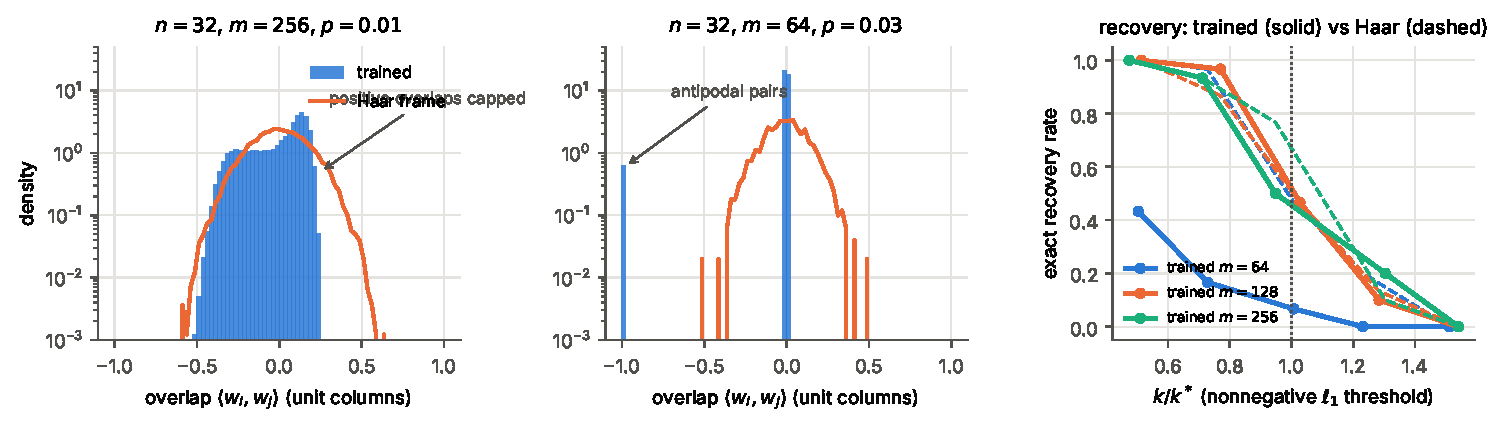
\includegraphics[width=\linewidth]{figs/e02_tms.pdf}
\caption{E02. Left: overlaps between trained feature directions (bars) and between Haar-frame directions (line)
for $m=256$, $p=0.01$; trained codes are platykurtic, with fewer large overlaps. Middle: $m=64$; the trained code is
32 antipodal pairs. Right: exact recovery of nonnegative $k$-sparse combinations by $\ell_1$ minimization, trained
vs Haar, with the predicted threshold $k^*$ (dashed).}
\label{fig:e02}
\end{figure}
Three findings. (i) Every trained code is an essentially exact tight frame, so by \cref{prop:frame-identity} its
second moment \emph{must} match Haar; it does, to three digits. (ii) Beyond second order the trained codes are not
Haar. With $m=2n$ they are $n$ antipodal pairs---excess kurtosis $\approx60$, coherence $1$---a highly structured
code that is ideal for nonnegative features and a ReLU readout and terrible for signed ones. With $m=8n$ they are
\emph{better} than Haar at the extremes: negative excess kurtosis and lower coherence. Training finds structured
codes, as engineers do; the random code is the floor. (iii) On the task they were trained for, trained codes beat
the best uniformly-biased Haar frame by large factors, yet their $\ell_1$ recovery thresholds are close to the
Haar threshold and to the statistical-dimension prediction, consistent with the universality of that
threshold~\cite{Monajemi}.

\subsection{E03: language-model embeddings}
We extracted the RoBERTa-base~\cite{RoBERTa} token embedding matrix ($m=50{,}261$ tokens, $n=768$) and GloVe
100d~\cite{GloVe} ($m=400{,}000$, $n=100$) and treated vocabulary items as features. Each is analysed raw, centred
(mean removed) and whitened (multiplied by $\Sigma^{-1/2}$, which forces a tight frame) (\cref{tab:e03},
\cref{fig:e03}).
\begin{table}[h]\centering\footnotesize
\resizebox{\linewidth}{!}{\begin{tabular}{@{}ll cc c cc cc c@{}}\toprule
 & & $n\,\E\cos^2$ & excess & & \multicolumn{2}{c}{$\Pr(|\cos|>t)$} & \multicolumn{2}{c}{max coherence} & tight- \\
model & version & (Haar $\approx1$) & kurt. & $t$ & observed & Gaussian & observed & Haar & ness \\\midrule
RoBERTa & raw & 2.70 & 2.77 & 0.2 & 4.9e-03 & 3.0e-08 & 0.81 & 0.17 & 0.35 \\
 & centred & 2.13 & 3.05 & 0.2 & 2.5e-03 & 3.0e-08 & 0.81 & 0.17 & 0.43 \\
 & whitened & 0.99 & 5.09 & 0.2 & 2.9e-04 & 3.0e-08 & 0.88 & 0.17 & 0.85 \\
\addlinespace
GloVe & raw & 4.77 & -0.26 & 0.5 & 1.7e-02 & 5.7e-07 & 0.96 & 0.55 & 0.20 \\
 & centred & 1.53 & 0.64 & 0.5 & 9.1e-04 & 5.7e-07 & 0.98 & 0.55 & 0.65 \\
 & whitened & 1.02 & 0.42 & 0.5 & 2.0e-04 & 5.7e-07 & 0.94 & 0.55 & 0.96 \\
\bottomrule\end{tabular}}

\medskip
\resizebox{0.6\linewidth}{!}{\begin{tabular}{@{}lrr ccc@{}}\toprule
 & & & \multicolumn{3}{c}{exact $\ell_1$ recovery rate} \\
model & $m_{\rm sub}$ & $k$ ($k^*$) & centred & whitened & Haar \\\midrule
RoBERTa & 1536 & 222 (296) & 1.00 & 1.00 & 1.00 \\
RoBERTa & 1536 & 296 (296) & 0.50 & 0.50 & 0.62 \\
RoBERTa & 1536 & 370 (296) & 0.00 & 0.00 & 0.00 \\
GloVe & 200 & 19 (39) & 1.00 & 1.00 & 1.00 \\
GloVe & 200 & 29 (39) & 1.00 & 1.00 & 0.97 \\
GloVe & 200 & 35 (39) & 0.83 & 0.93 & 0.83 \\
GloVe & 200 & 39 (39) & 0.57 & 0.47 & 0.43 \\
GloVe & 200 & 42 (39) & 0.23 & 0.27 & 0.30 \\
GloVe & 200 & 48 (39) & 0.00 & 0.00 & 0.03 \\
\bottomrule\end{tabular}}
\caption{E03: language-model embeddings as codes. Top: overlap statistics over $4\times10^5$ random pairs; $t$ is the tabulated threshold nearest $4/\sqrt n$ ($5.5/\sqrt n$ for RoBERTa, $5/\sqrt n$ for GloVe);
the Gaussian column is the tail of $\mathcal N(0,1/n)$; coherence over 4000 random items. Bottom: signed $\ell_1$
recovery from a random sub-dictionary of $m_{\rm sub}=2n$ items ($k^*$: predicted threshold; RoBERTa 8 trials per
entry, GloVe 30).}
\label{tab:e03}\end{table}

\begin{figure}[t]
\centering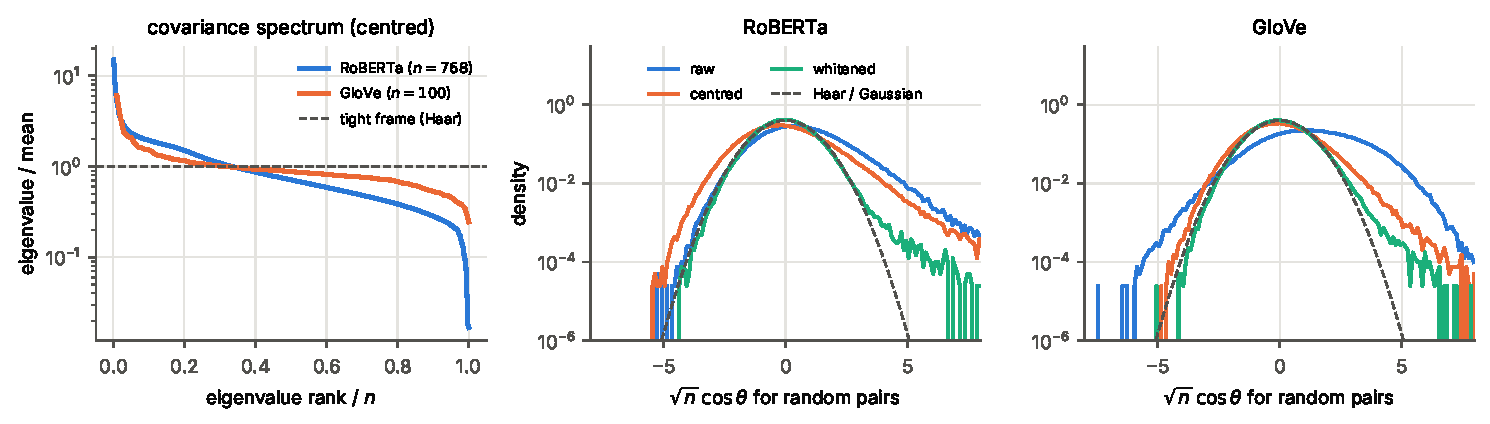
\includegraphics[width=\linewidth]{figs/e03_embeddings.pdf}
\caption{E03. Left: covariance spectra of centred embeddings, normalized to mean one; a Haar (tight) frame is the
flat line. Middle and right: distribution of $\sqrt n\cos\theta$ for random pairs, raw, centred and whitened, against
the Haar/Gaussian prediction (dashed). Whitening restores the bulk; the tails remain heavy.}
\label{fig:e03}
\end{figure}
Real embeddings depart from Haar in two layers. The first is \emph{anisotropy}: a common mean direction and a
spectrum far from flat, so the frame is far from tight and the mean-square overlap is several times the Haar value
(a known property of language-model embeddings~\cite{Ethayarajh}). Whitening removes this by construction and
returns the second moment to $1/n$ (again by \cref{prop:frame-identity}). The second layer survives whitening: the
\emph{tails} of the overlap distribution are far heavier than Gaussian. Listing the most coherent pairs
(\file{scripts/e03\_top\_pairs.py}) shows what they are. In RoBERTa they are the same word with and without a
leading space or capital (``As''/``\,As'', ``Georgia''/``\,Georgia'', ``Education''/``education''), inflections
(``turned''/``turning'', ``tend''/``tends'') and near-synonyms (``spokesman''/``spokeswoman'',
``Usually''/``Normally''), with $\abs{\cos}\approx0.7$--$0.9$. In GloVe they are rare tokens of one type: numbers
(``28.6''/``24.9'', ``1679''/``1677'', ``84-year''/``83-year''), Polish place names, moth genera. Either way they
are not independent features at all. Nevertheless the bulk
behaves like a random code: $\ell_1$ recovery of random sparse combinations from a random sub-dictionary with $m=2n$
sits at the Haar threshold.

Two cautions keep this last result in proportion. First, it is less surprising than it looks: the Donoho--Tanner
transition is known to be universal well beyond Gaussian matrices, including for many deterministic
frames~\cite{Monajemi}, and we are seeing one more instance. Second, our test draws random supports, which is the
typical case where agreement is expected. Real activations co-activate correlated features (the near-duplicates
above), and a random-support test cannot see that. The embeddings tested are input embeddings; dictionaries of
internal representations (sparse autoencoders on a residual stream) are the test that matters most and were not
reachable here.

\subsection{What this means for the correspondence}\label{sec:part1-meaning}
The Haar code is the right null model and the wrong description. Statements about \emph{typical} sparse sets
(recovery thresholds, the restricted isometry of random supports) transfer from Haar codes to trained ones,
because they depend on second-order structure, which tight frames share. Statements about \emph{worst-case} sets
(coherence, the cheapest null vector) do not: trained codes can be better than random (toy models with plentiful
features) or much worse (embeddings with near-duplicates). In black hole language, a trained code is a designed
error-correcting code rather than a scrambler's typical one---which raises the question, not pursued here, of
whether a black hole's actual code (as opposed to its Haar model) has analogous structure.
